%
% Tutorial -- DC and AC Analysis, Parameter Sweep and Device Models
%
% Copyright (C) 2005 Stefan Jahn <stefan@lkcc.org>
% Copyright (C) 2005 Chris Pitcher <ozjp@chariot.net.au>
%
% Permission is granted to copy, distribute and/or modify this document
% under the terms of the GNU Free Documentation License, Version 1.1
% or any later version published by the Free Software Foundation.
%

\documentclass[12pt,a4paper,oneside]{report}

% Include basic and title page definitions.
%
% This document contains a generic preamble for tutorials.
%
% Copyright (C) 2005 Stefan Jahn <stefan@lkcc.org>
%
% Permission is granted to copy, distribute and/or modify this document
% under the terms of the GNU Free Documentation License, Version 1.1
% or any later version published by the Free Software Foundation.
%

% Load some packages.
\newcommand{\tutpackages}{%
  \usepackage{savesym}
  \usepackage{a4wide}
  \usepackage[T1]{fontenc}
  \usepackage{longtable}
  \usepackage{ae,aecompl}
  \usepackage{url}
  \usepackage{epsfig}
  \usepackage{array}
  \usepackage{subfigure}
  \usepackage{amsmath}
  \usepackage{amsfonts}
  \savesymbol{iint}
  \usepackage{stmaryrd}
  \usepackage{wasysym}
  \restoresymbol{WASY}{iint}
  \usepackage{pifont}
  \usepackage[amssymb]{SIunits}
  \usepackage{graphics}
  \usepackage{psfrag}
  \usepackage{relsize}
  \usepackage[section]{placeins}
  \usepackage{listings}
}

% Compatibility code for LaTeX and pdfTeX.
\newcommand{\tutcompat}{%
  \newif\ifpdf
  \ifx\pdfoutput\undefined
    \pdffalse
  \else
    \pdfoutput=1
    \pdftrue
  \fi
}

% Only evaluated if run using pdfTeX.
\newcommand{\tutheader}[2]{%
  \ifpdf
    \usepackage[pdftex,
	a4paper,
	backref,
	\iftutbook
	  anchorcolor=black,
	  filecolor=black,
	  menucolor=black,
	  pagecolor=black,
	  bookmarks=true,
	  bookmarksopen=true,
	  bookmarksnumbered=true,
	  pdfpagemode=UseOutlines,
	\else
	  bookmarks=false,
	  bookmarksopen=false,
	  bookmarksnumbered=true,
	  pdfpagemode=UseNone,
	\fi
	baseurl={http://qucs.sourceforge.net},
	pdfstartview=FitH,
	pdftitle={Qucs - \tuttitle},
	pdfauthor={#2},
	pdfsubject={#1},
	colorlinks,
	linkcolor=black,
	urlcolor=black,
	citecolor=black,
	backref=false,
	plainpages=false,
	pagebackref=false]{hyperref}
    \DeclareGraphicsExtensions{.pdf,.png}
    \pdfcompresslevel 9
    \pdfinfo {
      /Title   (Qucs - \tuttitle)
      /Subject (#1)
      /Author  (#2)
    }
  \else
    \DeclareGraphicsExtensions{.eps}
  \fi
  \graphicspath{{pics/}}
}

% Generic tutorial startup code.
\newcommand{\tutstartup}[2]{%
  \tutpackages
  \tutcompat
  \tutheader{#1}{#2}
}

% Begin document.
\newcommand{\tutbegin}{%
  \begin{document}
  \tuttitlepage
  \setlength{\parindent}{0pt}
}

% End document.
\newcommand{\tutend}{%
  \end{document}
}

%
% This document contains a generic title page for tutorials.
%
% Copyright (C) 2005, 2006 Stefan Jahn <stefan@lkcc.org>
%
% Permission is granted to copy, distribute and/or modify this document
% under the terms of the GNU Free Documentation License, Version 1.1
% or any later version published by the Free Software Foundation.
%

% Title page definitions.
\newcommand{\tuttitlepage}{%
  \makeatletter
  \begin{titlepage}
    \setlength{\parindent}{0pt}
    \vspace*{3cm}
    \begin{flushleft}
      \textbf{\begin{huge} Qucs \end{huge}}
    \end{flushleft}
    \hrule height 3pt
    \begin{flushright}
      \begin{LARGE} \tuttitle\\ \end{LARGE}
      \if\empty\tutsubtitle\else
        \vspace*{12pt}
        \begin{Large} \tutsubtitle \end{Large}
      \fi
    \end{flushright}
    \vfill
    \begin{flushright}
      \begin{Large} \tutauthor \end{Large}
    \end{flushright}
    \hrule height 3pt
    \vspace*{24pt} \tutcopyright \vspace*{12pt}

Permission is granted to copy, distribute and/or modify this document
under the terms of the GNU Free Documentation License, Version 1.1 or
any later version published by the Free Software Foundation.  A copy
of the license is included in the section entitled "GNU Free
Documentation License".

    \vspace*{1cm}
  \end{titlepage}
  \setcounter{footnote}{0}
  \makeatother
}

% Extra command for tutorial definitions.
\newcommand{\tutauthor}[1]{\def\tutauthor{#1}}
\newcommand{\tutcopyright}[1]{\def\tutcopyright{#1}}
\newcommand{\tuttitle}[1]{\def\tuttitle{#1}}
\newcommand{\tutsubtitle}[1]{\def\tutsubtitle{#1}}

% WorkBook conditional.
\newif\iftutbook
\tutbookfalse

% Section redefinitions.
\newcommand{\tutsection}[1]{%
  \iftutbook
    \section{#1}
  \else
    \section*{#1}
  \fi
}
\newcommand{\tutsubsection}[1]{%
  \iftutbook
    \subsection{#1}
  \else
    \subsection*{#1}
  \fi
}
\newcommand{\tutsubsubsection}[1]{%
  \iftutbook
    \subsubsection{#1}
  \else
    \subsubsection*{#1}
  \fi
}
\newcommand{\tutparagraph}[1]{%
  \iftutbook
    \paragraph{#1}
  \else
    \paragraph*{#1}
  \fi
}
\newcommand{\tutsubparagraph}[1]{%
  \iftutbook
    \subparagraph{#1}
  \else
    \subparagraph*{#1}
  \fi
}


\tuttitle{
  A Tutorial}
\tutsubtitle{
  DC and AC Analysis, Parameter Sweep and Device Models}
\tutauthor{
  Stefan Jahn\\
  Chris Pitcher\vspace*{6pt}\\
  Juan Carlos Borr�s}
\tutcopyright{
  Copyright \copyright{} 2005 Stefan Jahn
  \textless stefan@lkcc.org\textgreater\\
  Copyright \copyright{} 2005 Chris Pitcher
  \textless ozjp@chariot.net.au\textgreater\\
  Copyright \copyright{} 2007 Juan Carlos Borr�s
  \textless jcborras@gmail.com\textgreater}
\tutbookfalse

\tutstartup{\tutsubtitle}{Chris Pitcher and Stefan Jahn and Juan Carlos Borr�s}

% Here finally starts everything.
\tutbegin

%
% Tutorial -- DC analysis, Parameter sweep and Device models
%
% Copyright (C) 2005 Stefan Jahn <stefan@lkcc.org>
% Copyright (C) 2005 Chris Pitcher <ozjp@chariot.net.au>
%
% Permission is granted to copy, distribute and/or modify this document
% under the terms of the GNU Free Documentation License, Version 1.1
% or any later version published by the Free Software Foundation.
%

\tutsection{DC Static Circuits}

A favourite question in electronics courses used to be:

\begin{quotation}
\textit{You have twelve one ohm resistors; you connect them together
so that each resistor lies along the edge of a cube. What is the
resistance between opposite corners of the cube?}
\end{quotation}

The intention may have been to teach soldering, as more than one
student solved it by making just such a cube! These days we can do
that without touching the soldering iron; we simulate the circuit.

\addvspace{12pt}

Here is my attempt to make a cube in Qucs; anyone is welcome to try
and improve it.

\begin{figure}[ht]
  \centering
  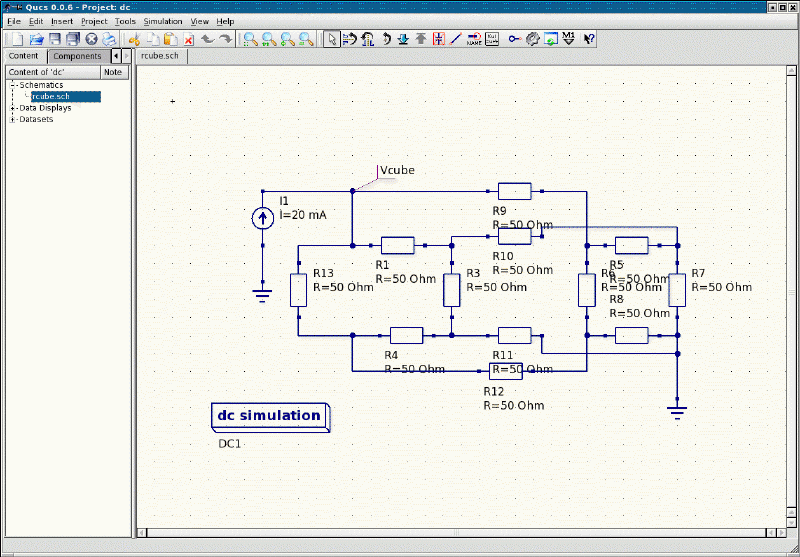
\includegraphics[width=1\linewidth]{rcubesch}
  \caption{resistor cube schematic}
  \label{fig:rcubesch}
\end{figure}
\FloatBarrier

All I did was select resistance in the left hand component window and
paste them down, rotating as necessary, until I had twelve on the
schematic.  Then I wired two sets of four into squares, then connected
the remaining four between the corners of the squares.  Which I'm sure
is topologically the same as a cube.

\addvspace{12pt}

Which all might seem trivial, but is a good reminder right at the
beginning that we are creating a virtual representation of a physical
circuit.  Sometimes we have to bend and squeeze things to get it into a
format that our simulator will accept, which leaves us wondering
whether we are working with an accurate representation.

\addvspace{12pt}

\textbf{The Rule} is: if we can correlate the junctions of our
components with those of the real circuit, we are accurately
representing the physical circuit.  And, I might add, it is ALWAYS
worth checking that we have done it right; simulate the wrong circuit
and it will tell you lies.

\addvspace{12pt}

With my cube of resistors accurately drawn, I only have to hit the
simulation button and the tabulated results will show me the voltage
at the corner node.  As I am forcing a constant current through the
cube from one corner to another, Ohm's Law tells me that the voltage
between those corners will give me the resistance.  If I use a current
of one amp, the output voltage will be equal to the resistance in
ohms.\footnote{I could tell you the value my simulation gave, but why
should I spoil your fun.... go ahead and run it yourself. If you
really want to be thorough you could then also build the circuit and
measure the result.....}

\addvspace{12pt}

Those with good attention to detail will be complaining about now that
I haven't really solved the problem, as the question mentioned one ohm
resistors while I have used fifty ohms.  Well, yes, I cheated.  Which
I often do in simulations.

\addvspace{12pt}

To set all the resistances to the correct value I would have had to
open the Properties Editor window twelve times; here is how it
looks...

\begin{figure}[ht]
  \centering
  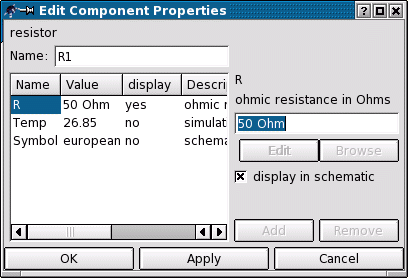
\includegraphics[width=0.7\linewidth]{propeditrwin}
  \caption{component property dialog}
  \label{fig:propeditrwin}
\end{figure}
\FloatBarrier

and the highlighted value is inviting me to type in an alternative. I
could have done this, but natural laziness got the better of me. I
reasoned that fifty ohms is fifty times too high, but if I reduced the
current source from one amp to twenty milliamps, the output voltage
would be the same.  You will find such laziness (or acute perception,
depending on is telling the story!) can save much time and effort.

\tutsection{When Things Vary}

All of which is interesting, but not nearly as interesting as when we
start changing things like the supply voltage and see the effects. For
linear devices with a DC supply, the answer would be: not much.  It's
when we introduce non-linear elements that things start to happen.

\addvspace{12pt}

The simplest non-linear element is the diode, and the question we ask
most often about a diode is: how does the diode forward voltage vary
with current? So back to Qucs and draw this circuit...

\begin{figure}[ht]
  \centering
  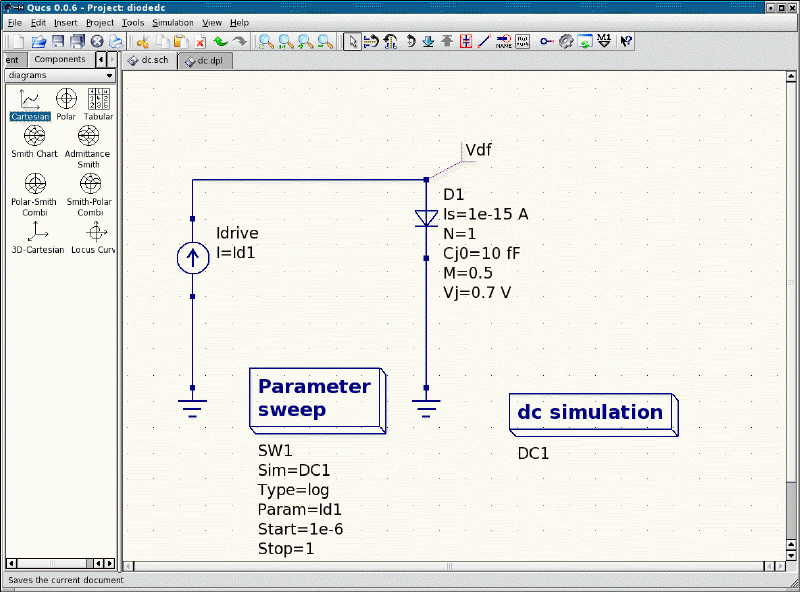
\includegraphics[width=1\linewidth]{diodedcsch}
  \label{fig:diodedcsch}
\end{figure}
\FloatBarrier

This circuit looks deceptively simple, but it introduces a few more
features of Qucs, so let's go through them in order.

\addvspace{12pt}

The components were again selected from the left hand window and wired
together. Then the two boxes were selected from the
\textbf{simulations} window.

\addvspace{12pt}

The DC simulation box can be pretty much left as is for now, but take
note of the name of the simulation: \textbf{DC1}.

\addvspace{12pt}

The \textbf{Parameter sweep} box properties dialog looks like this
when opened...

\begin{figure}[ht]
  \centering
  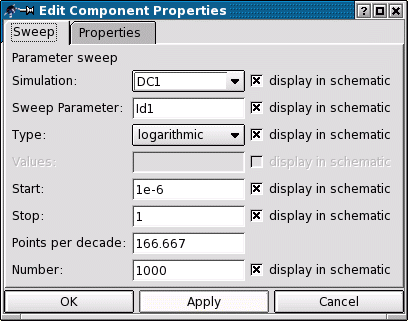
\includegraphics[width=0.7\linewidth]{sweepedit}
  \label{fig:sweepedit}
\end{figure}
\FloatBarrier

The first two items to take note of are the \textbf{Simulation} entry
(here \textbf{DC1}, corresponding to the name of the simulation box)
and the \textbf{Sweep Parameter} entry, here entered as \textbf{Id1}.
If you look at the current source driving our diode you will see that
it just happens to be labeled \textbf{Idrive}.  So the result of all
this is that the component property value \textbf{Id1} of the current
source's property \textbf{I} will be swept through a range of values
as determined by our parameter sweep function named
\textbf{SW1}.\footnote{You can change this name if you wish, in the
Properties menu of the Edit properties window.}

\addvspace{12pt}

The rest of the entries set the type of sweep (here logarithmic) and
the range of values over which to sweep. You can try different values
in any of these to see the effect; one of the advantages of a
simulator over a physical prototype is that you can't blow up your
diode by feeding too much current through it!

\addvspace{12pt}

So I hit the simulation button and it passed me over the results page,
and I created a couple of graphs of the output.  This is how my screen
looked...

\begin{figure}[ht]
  \centering
  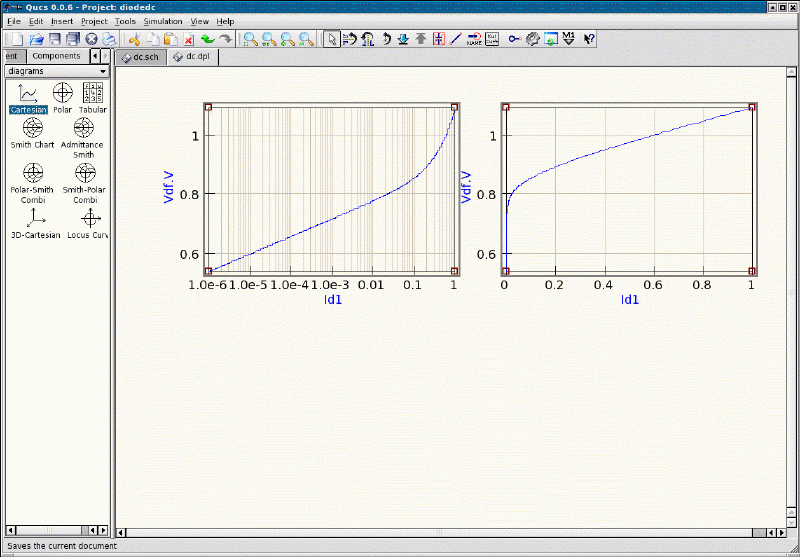
\includegraphics[width=1\linewidth]{diodedcop}
  \label{fig:diodedcop}
\end{figure}
\FloatBarrier

In each case I have a plot of diode forward voltage (Y-axis) against
forward current (X-axis).  The left hand graph has a logarithmic scale
for forward current, while the right hand graph uses a linear current
scale.  How did I do that? Well, you should know by now that all
things are easy with Qucs!

\addvspace{12pt}

When you select a graph type from the left hand window and drag it
into the viewing area, it creates a graph and opens a dialog which
looks like this
\begin{figure}[ht]
  \centering
  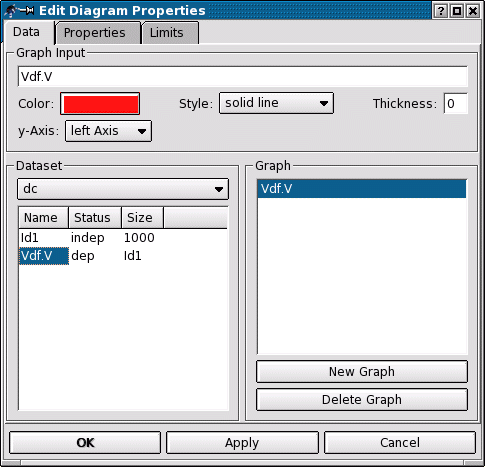
\includegraphics[width=0.7\linewidth]{grapheditd}
  \label{fig:grapheditd}
\end{figure}
\FloatBarrier

The left hand window shows the available variables and whether they
are dependent or independent. Here the current Id1 is the independent
variable, and the forward voltage Vdf.V is the dependent. Double-click
on the entry for Vdf.V and it is transferred to the right hand side;
hit OK and the graph will be drawn.

\addvspace{12pt}

That should give you something like the right hand graph in my
screenshot above.  Do it all again, but this time before clicking OK
open the Properties window, which looks like this.
\begin{figure}[ht]
  \centering
  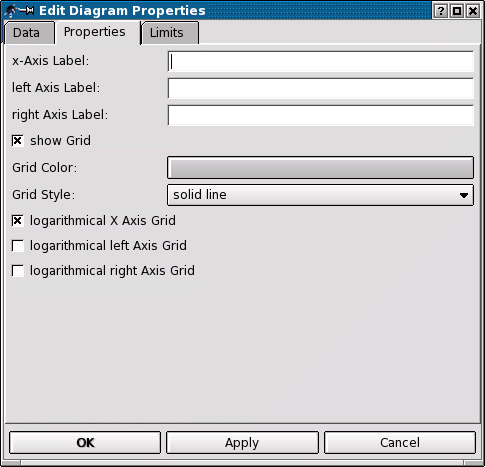
\includegraphics[width=0.7\linewidth]{grapheditp}
  \label{fig:grapheditp}
\end{figure}
\FloatBarrier

Here I've selected a logarithmic X Axis, which gave me the graph on
the left hand side.  I've also moved them around and re-sized them to
pretty them up; you can do all kinds of fancy things if you want.

\addvspace{12pt}

Now I've sneaked in another test to see if you are really following
this. Those of you who did run this simulation are probably wondering
about now why your graphs look rather different to mine. In
particular, at high currents on the logarithmic scale your curve is a
straight line, while mine curves upwards alarmingly. What is happening
?

\addvspace{12pt}

What I did was open the Properties dialog for the diode and set some
parameters.  This is what the dialog box looks like...

\begin{figure}[ht]
  \centering
  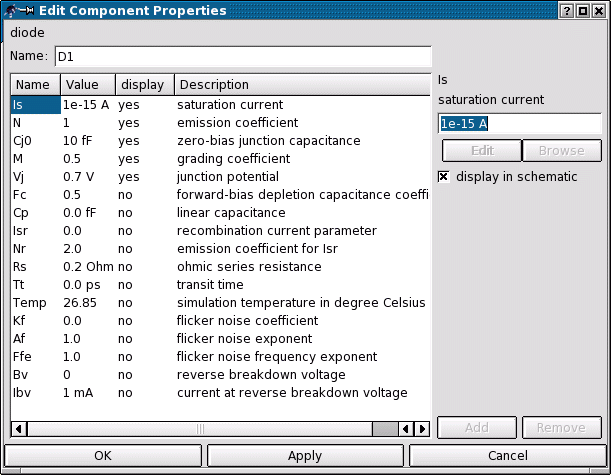
\includegraphics[width=0.8\linewidth]{diodeditprop}
  \label{fig:diodeditprop}
\end{figure}
\FloatBarrier

and each of these entries sets one parameter of the virtual component
we are using to model the diode.

\addvspace{12pt}

So, what are these parameters? Time to explore one of the delights of
computer circuit simulation, device modeling...

\tutsection{Models and Parameters}

When the computer creates that small piece of virtual reality which
represents your physical circuit, it uses sets of equations which
describe the operation of each device you insert. The equation which
relates the diode DC forward voltage as a function of current is
\begin{equation*}
I_d = I_s\cdot\left(e^{\tfrac{V_d}{n\cdot V_t}} - 1\right)
\end{equation*}

where $V_t$ is the forward voltage drop at 25 degrees C of an ideal
junction, also given by
\begin{equation*}
V_t = \dfrac{k_B\cdot T}{q}
\end{equation*}

where
\begin{align*}
k_B &= \textrm{Boltzmann's constant}\\
T &= \textrm{temperature in degrees Kelvin}\\
q &= \textrm{charge of the electron}
\end{align*}

most of these are constants that the program already knows about. The
ones we need to supply are the ones listed in the properties editor
window. For the DC characteristics, most of the time, the only ones we
need to worry about are Is, the saturation current, and T, the
temperature. If we are going to push relatively high currents through
the diode we can also include an estimate for the series resistance
Rs; if we are worried about low current behaviour then we need to add
the reverse current parameter Isr.

\addvspace{12pt}

How do we know what values to insert? Much could be written about
device modeling; much indeed has been written about device modeling.
As always, we really have two choices: use a value from someone else,
or find our own values, usually by trial and error.

\addvspace{12pt}

There are a great many models available for various simulation
programs. Probably the most freely available are those for spice, many
of which can be downloaded from the semiconductor companies. Here, for
example, is a typical spice model for a 1N4148 diode:\footnote{I don't
know where this came from, so I can't acknowledge the author. Most
libraries are copyright, even if freely available.}

\begin{verbatim}
        .model 1N4148  D(Is=0.1p Rs=16 CJO=2p Tt=12n Bv=100 Ibv=0.1p)
        85-??-??   Original library
\end{verbatim}

Any values not supplied are assumed to be the defaults.

\addvspace{12pt}

The other way is to create your own device parameters, which is a bit
like catching worms before you can go fishing. Insert values, plot the
resulting characteristics, see how they compare with the published
data sheet values, go back and adjust the values; continue until
satisfied or exhausted.

\addvspace{12pt}

Here, for example, is a circuit for quickly comparing the forward
characteristics of diodes with different parameter values.
\begin{figure}[ht]
  \centering
  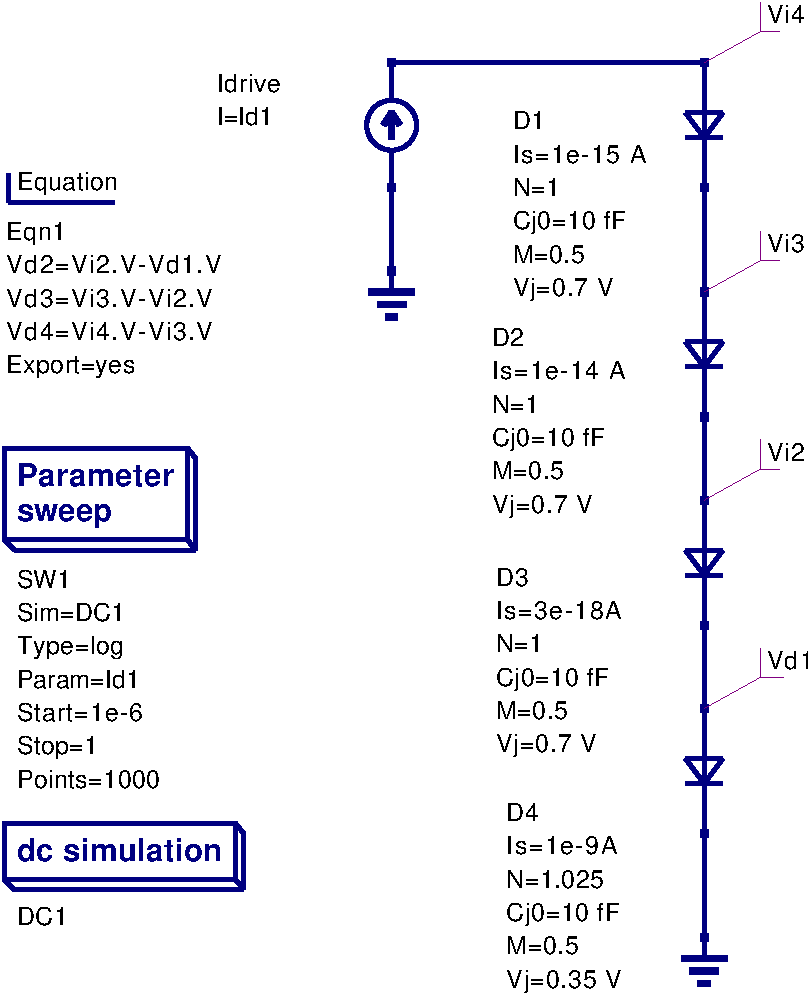
\includegraphics[width=0.45\linewidth]{diod4schr}
  \label{fig:diod4schr}
\end{figure}
\FloatBarrier

And here is the plotted output...
\begin{figure}[ht]
  \centering
  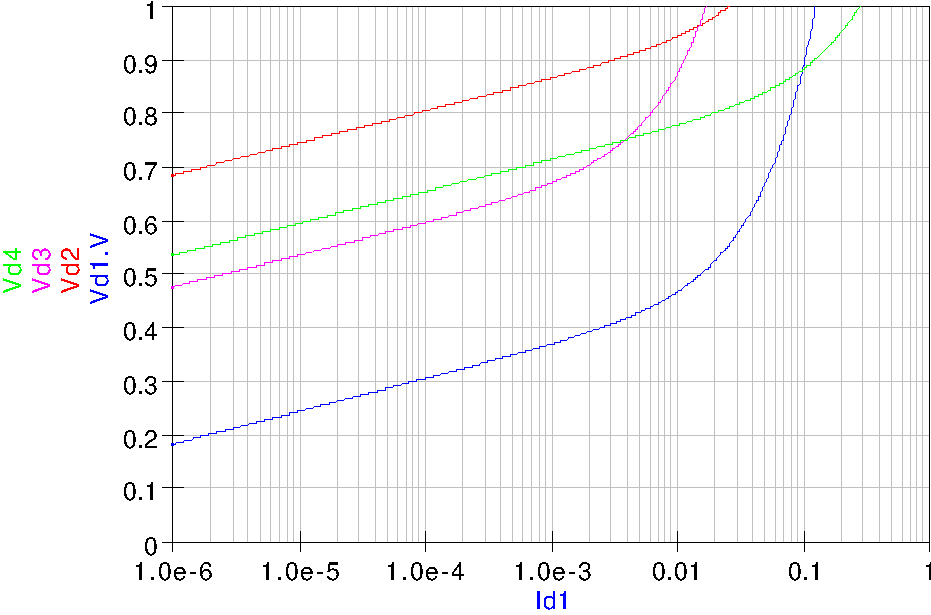
\includegraphics[width=0.55\linewidth]{diod4out}
  \label{fig:diod4out}
  \caption{Diode Forward Voltage}
\end{figure}
\FloatBarrier

The green and purple curves are typical of 1N4148 and 1N4448 devices;
the others are medium and low-barrier Schottky devices. I have done a
first pass compare with the data sheets, but I can't guarantee that
these curves are any more than my best estimates.\footnote{I'm
assuming you are sick of screenshots by now, so I've just printed the
schematic and display files from Qucs; you'll find the print item in
the file menu, and if you ask it nicely it will print a postscript
file.}

\addvspace{12pt}

If you want to know more details of what each parameter does, there
has been a great deal written over the years, particularly for spice,
on the subject; a google search will quickly reveal most of it.  Qucs
comes with a document which lists the details of its models, and,
being open source, there is always the code itself.

\addvspace{12pt}

Most of us end up taking a great deal on trust, and matching curves to
data sheets as best we can.  This is yet another instance of one of
the fundamentals of engineering, the Duck Principle\footnote{Usually
expressed as: If it looks like a duck, walks like a duck, quacks like
a duck and tastes like a duck, then, for all practical purposes, it is
a duck.}: If you can't detect any difference between the behaviour of
your model and the physical device, then they are, for engineering
purposes, the same. Put it another way, when the difference between
the model and the real device drops below the usual level of
measurement uncertainty, it does matter any more.

\addvspace{12pt}

In any case, component spreads in the real world tend to make the fine
details of model inaccuracies somewhat academic, as we shall see when
we model more complex devices.


\tutend
